\clearpage % Rozdziały zaczynamy od nowej strony.

\section{Wdrożenie}

Aby zapewnić sprawne działanie systemu mikroserwisowego, należy zadbać o odpowiednie środowisko uruchomieniowe, w którym będą działać poszczególne komponenty. Ponadto, należy zapewnić odpowiednie narzędzia, które pozwolą na automatyzację procesu wdrażania nowych wersji oprogramowania.

\subsection{CI/CD}

Jednym z narzędzi, które mogą usprawnić proces wdrażania oprogramowania, jest CI/CD, czyli ciągła integracja i ciągłe wdrażanie. CI/CD pozwala na automatyzację procesu budowania aplikacji, testowania jej, a następnie wdrażania do środowiska produkcyjnego.

W ramach pracy inżynierskiej został zaimplementowany potok CI/CD w ramach platformy GitHub Actions. Przykładowo, dla serwisu serwerowego potok ten składa się z następujących kroków:

\begin{enumerate}
    \item Przygotowanie środowiska z zainstalowanymi JDK 21 i Gradle \cite{gradle} 8.1.1
    \item Przeprowadzenie analizy statycznej kodu za pomocą narzędzia Detekt \cite{detekt}
    \item Przeprowadzenie testów jednostkowych i integracyjnych (komenda \texttt{./gradlew test})
    \item Zbudowanie aplikacji za pomocą Gradle (komenda \texttt{./gradlew build})
    \item Zbudowanie obrazu Docker za pomocą Docker Buildx (komenda \texttt{docker buildx build})
    \item Opublikowanie zbudowanego obrazu w GitHub Container Registry \cite{ghcr} (komenda \texttt{docker push})
    \item (opcjonalnie) Wdrożenie zbudowanego obrazu na klastrze Kubernetes (komenda \texttt{kubectl apply})
\end{enumerate}

Wszystkie komponenty systemu są budowane równolegle, co pozwala na skrócenie czasu budowania całego systemu. W przypadku, gdy któryś z kroków zakończy się niepowodzeniem, proces budowania zostaje przerwany, a programista otrzymują informację o błędzie.

Na listingu \ref{lst:deployment-cicd} przedstawiono fragment pliku konfiguracyjnego potoku CI/CD dla serwisu serwerowego z pominięciem mniej istotnych kroków.

\begin{lstlisting}[caption={Fragment potoku CI/CD},label={lst:deployment-cicd},captionpos=b,numbers=left]
name: Build & Publish
on:
  push:
    branches:
      - master
    tags:
      - "v[0-9]+.[0-9]+.[0-9]+"
  pull_request:
    branches:
      - master
jobs:
  build-services:
    runs-on: ubuntu-latest
    strategy:
      matrix:
        service: [restaurant, order, payment, delivery, query, saga]
    steps:
      - uses: actions/checkout@v3
      - name: Set up JDK
        uses: actions/setup-java@v3
      - name: Set up Gradle
        uses: gradle/gradle-build-action@v2
      - name: Build with Gradle
        run: ./gradlew build
      - name: Build and push
        uses: docker/build-push-action@v4
        with:
          context: ./${{ matrix.service }}
          push: true
          platforms: linux/amd64,linux/arm64
\end{lstlisting}

W przypadku implementowanego systemu wykonanie całego potoku wraz z wdrożeniem trwa około 3 minuty.

\subsection{Repozytorium artefaktów}

Aby umożliwić uruchomienie dowolnego elementu systemu przez programistów, należy zagwarantować dostępność wymaganych artefaktów. W przypadku implementowanego systemu artefaktem tym jest moduł \textit{shared}, który jest wymagany przez wszystkie inne usługi. W tym celu wykorzystano GitHub Actions Artifacts \cite{gaa}, które umożliwiają przechowywanie artefaktów np. systemu budowania Gradle i są zintegrowane z potokiem CI/CD.

\subsection{Konteneryzacja}

Wdrażanie systemów mikroserwisowych z wykorzystaniem technologii Docker stało się standardem w rozwoju nowoczesnych aplikacji webowych. Docker umożliwia tworzenie lekkich, przenośnych kontenerów dla każdego mikroserwisu, które zapewniają izolację i niezależność dla każdego mikroserwisu. Każdy kontener zawiera wszystkie niezbędne składniki (kod, środowisko wykonawcze, biblioteki), co umożliwia mikroserwisowi działać spójnie i niezawodnie w różnych środowiskach. 

Na listingu \ref{lst:deployment-docker} przedstawiono plik konfiguracyjny Dockerfile dla serwisu serwerowego.

\begin{lstlisting}[caption={Instrukcja budowania obrazu Docker serwisu serwerowego},label={lst:deployment-docker},captionpos=b,numbers=left]
FROM amazoncorretto:21
VOLUME /tmp
COPY build/libs/*.jar app.jar
ENTRYPOINT ["java","-jar","/app.jar"]
\end{lstlisting}

Budowa obrazu na jego podstawie polega na skopiowaniu pliku \texttt{.jar} z kodem aplikacji do kontenera, a następnie uruchomieniu go. Dzięki temu, że obraz jest budowany na podstawie gotowego obrazu \texttt{amazoncorretto:21}, który bazuje na dystrybucji OpenJDK od firmy Amazon, nie jest wymagane samodzielne instalowanie JDK.
    
\subsection{Orkiestracja kontenerów}

W celu zapewnienia skalowalności i niezawodności systemu mikroserwisowego, należy zadbać o odpowiednie narzędzia do orkiestracji kontenerów. W przypadku implementowanego systemu wykorzystano narzędzie Kubernetes \cite{k8s}, które umożliwia automatyzację wdrażania, skalowania i zarządzania aplikacjami kontenerowymi.

Kubernetes pozwala na uruchomienie wielu instancji każdego mikroserwisu, które mogą być automatycznie skalowane w zależności od obciążenia. Ponadto, Kubernetes zapewnia automatyczne wdrażanie nowych wersji oprogramowania, dzięki czemu nie jest wymagane ręczne uruchamianie nowych kontenerów. Ponadto, obsługuje on mechanizmy zcentralizowanej konfiguracji, woluminów dyskowych, monitorowania aplikacji oraz obsługi sieci.

Narzędzie to oferuje deklaratywne podejście do konfiguracji, co oznacza, że użytkownik określa stan, w którym powinien znajdować się system, a Kubernetes automatycznie dokonuje niezbędnych zmian, aby osiągnąć zadany stan. W przypadku implementowanego systemu stan systemu jest określony za pomocą plików YAML, które opisują wymagane zasoby, takie jak kontenery, woluminy, sieci itp.

\begin{lstlisting}[caption={Fragment pliku konfiguracyjnego Kubernetes dla serwisu zamówień},label={lst:deployment-k8s},captionpos=b,numbers=left]
apiVersion: apps/v1
kind: Deployment
metadata:
  name: order-service
spec:
  replicas: 1
  selector:
    matchLabels:
      app: order-service
  template:
    metadata:
      labels:
        app: order-service
    spec:
      containers:
        - env:
            - name: AXON_AXONSERVER_SERVERS
              value: axonserver
            - name: AXONIQ_CONSOLE_CREDENTIALS
              value: "XXX"
            - name: SPRING_PROFILES_ACTIVE
              value: gmaps
            - name: GMAPS_API_KEY
              valueFrom:
                secretKeyRef:
                  name: gmaps-api-key
                  key: key
          image: ghcr.io/bartlomiejrasztabiga/thesis/order:0.21.3
          name: order-service
          ports:
            - containerPort: 8102
          livenessProbe:
            httpGet:
              path: /actuator/health/liveness
              port: 8102
            initialDelaySeconds: 30
            periodSeconds: 10
          readinessProbe:
            httpGet:
              path: /actuator/health/readiness
              port: 8102
            initialDelaySeconds: 30
            periodSeconds: 10
          resources:
            requests:
              memory: "250Mi"
              cpu: "125m"
      restartPolicy: Always
\end{lstlisting}

Oprócz podanego na wycinku \ref{lst:deployment-k8s} tzw. \textit{deploymentu}, który definiuje wymagane zasoby, należy zdefiniować również \textit{service}, który umożliwia komunikację sieciową.

Na podstawie powyższego pliku konfiguracyjnego, Kubernetes zapewni automatyczne wdrożenie jednej instancji serwisu zamówień w wersji 0.21.3, uruchomionego na porcie 8102 ze wstrzykniętymi podanymi zmiennymi środowiskowymi w sekcji \texttt{env}.

\subsection{Skalowanie}

Dzięki zastosowaniu orkiestratora kontenerów możliwe jest automatyczne skalowanie poszczególnych komponentów systemu, na podstawie podanych metryk np. średniego zużycia procesora lub pamięci RAM. W przypadku implementowanego systemu zastosowano ręczne skalowanie poziome poprzez zmianę parametru \textit{replicas}, czyli dodawanie lub usuwanie instancji serwisów w zależności od obciążenia, przez operatora systemu.

\subsection{Chmura Google Cloud Platform}

Produkcyjne wdrożenie systemu odbyło się w chmurze publicznej od firmy Google - Google Cloud Platform \cite{gcp}. Wdrożenie w chmurze publicznej pozwala na łatwe skalowanie zasobów, a także zapewnia wysoką dostępność systemu. Ponadto, chmura publiczna pozwala na łatwe wdrożenie systemu w różnych lokalizacjach geograficznych, co pozwala na zmniejszenie opóźnień sieciowych. 

Wybór ten został podyktowany również tym, że Autor nie dysponuje odpowiednią fizyczną infrastrukturą, która pozwoliłaby na wdrożenie systemu w środowisku lokalnym, biorąc pod uwagę wymagania systemu.

Google Cloud Platform posiada w swojej ofercie usługę Kubernetes Engine, która umożliwia uruchomienie zarządzanego klastra Kubernetes w chmurze. Wdrożenie systemu odbyło się na klastrze złożonym z trzech węzłów, które są uruchomione w strefie \textit{europe-central-2} (Warszawa, Polska). Każdy węzeł jest typu \textit{e2-standard-4}, co oznacza, że posiada 4 vCPU i 16 GB pamięci RAM oraz 100 GB przestrzeni dyskowej.

Domyślnie uruchomiono po jednej instancji serwisów obsługujących komendy (Dostawy, Zamówienia, Płatności, Restauracje) oraz po cztery instancje serwisów obsługujących większy ruch niż pozostałe (Zapytania oraz Sagi).

\subsection{Monitorowanie}

Do monitoringu systemu użyto kombinacji wbudowanych narzędzi Google Cloud Platform, zestawu narzędzi Grafana Loki \cite{grafana-loki} oraz platformy Axon Console \cite{axon-console}.

Grafana Loki jest narzędziem do agregacji i zbierania logów, które zostało zintegrowane z klastrem Kubernetes. Dzięki temu wszystkie logi z kontenerów są automatycznie zbierane i agregowane w jednym miejscu. Ponadto, dzięki integracji z platformą Grafana możliwe jest wizualizowanie, filtrowanie oraz wyszukiwanie logów w celach diagnostycznych.

Na rysunku \ref{fig:loki} przedstawiono przykładowe logi systemu w Grafana Loki.

\clearpage

\begin{figure}[!h]
    \centering 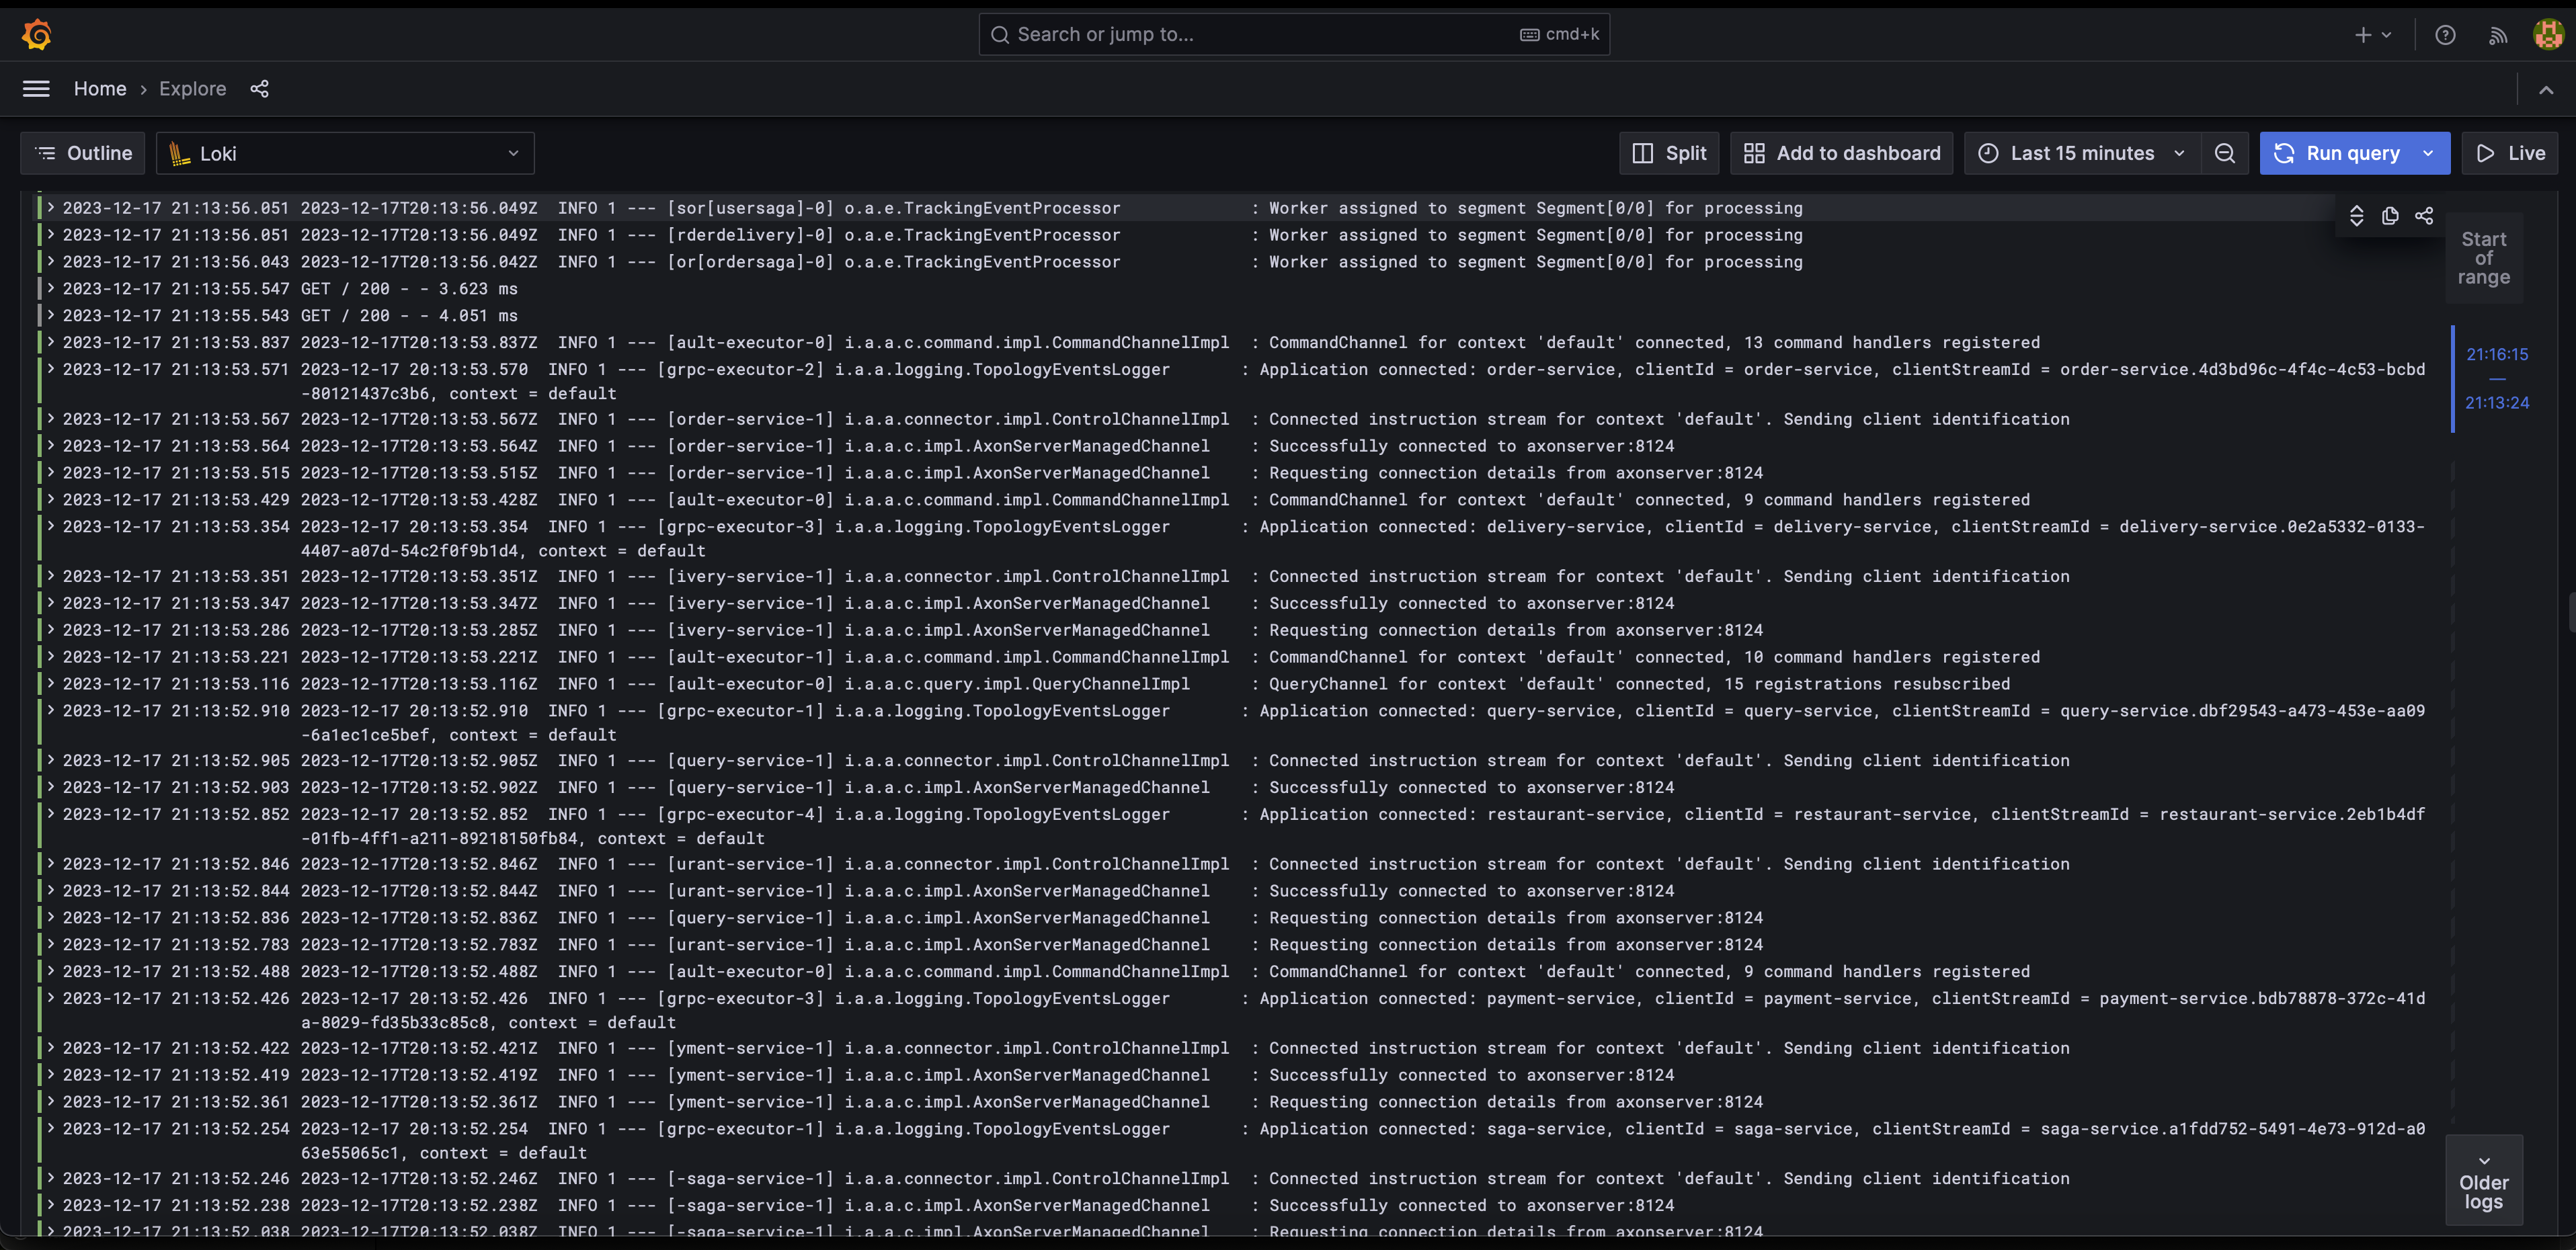
\includegraphics[width=1.0\linewidth]{loki.png}
    \caption{Logi systemu w Grafana Loki}
    \label{fig:loki}
\end{figure}

Axon Console jest platformą do monitorowania oraz zdalnego zarządzania systemami opartymi na frameworku Axon. Pozwala ona na wizualizację topologii systemu, monitorowanie stanu agregatów, zdarzeń, komend oraz zapytań, a także zarządzanie procesorami zdarzeń (np. dzielenie strumieni zdarzeń na partycje w celu równoległego procesowania).

Ponadto pozwala ona na monitorowanie średnich opóźnień w konsumpcji zdarzeń i liczby obsługiwanych komend na sekundę co pozwala na odnajdywanie wąskich gardeł w systemie.

Na rysunku \ref{fig:axonconsole} przedstawiono panel systemu Axon Console.

\begin{figure}[!h]
    \centering 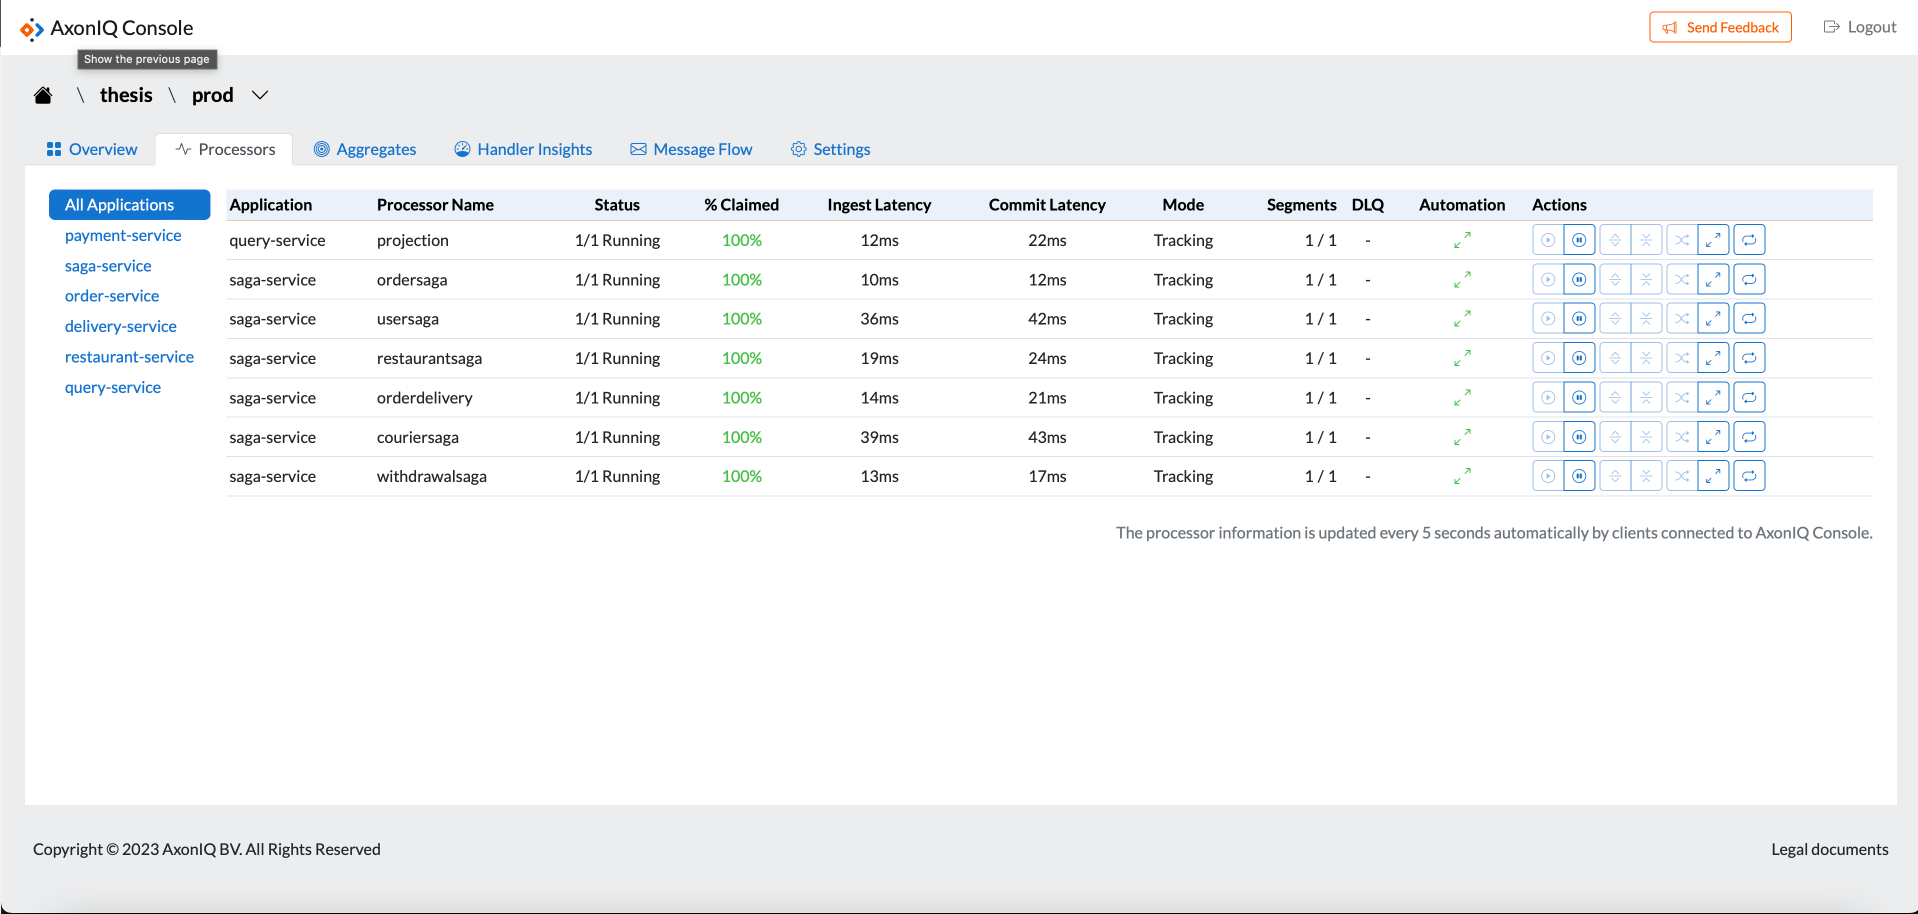
\includegraphics[width=1.0\linewidth]{axonconsole.png}
    \caption{Panel systemu Axon Console}
    \label{fig:axonconsole}
\end{figure}
